\chapter{Use Cases}
Before dipping into the concept and implementations of our two extensions, we present two examples to give readers a better understanding of problems encoded as workflows and the type of problems we are going to handle.

We present here two examples that are used to explore the semantics and performance of \dpy. We require to retain all prior semantic interpretations of workflows and PEs but introduce new ones that depend on dynamic determination of the generated graph.

We will introduce them separately for clarity.

\section{Prime Sieve} \label{sec:uc_sieve}
We first present \ttsieve which is a very simple yet useful algorithm. We present its basic idea, the common parallel algorithm for \ttsieve and the difficulty to construct it in the current semantics of \dpy (which is one of the motivations for our work).

The earliest known prime-number generating algorithm is \ttesieve given by Eratosthenes, an ancient Greek mathematician \cite{o2009genuine}. The basic idea of \ttesieve is that we cross out all multiples (up until a certain upper boundary) of every prime at the time we encounter a new prime.

As we are using prime sieves as demonstration, we mainly focus on the correctness and simplicity rather than the efficiency. Therefore, we can simply change the structure of \ttesieve into a distributed manner: each node is responsible for one prime, and it crosses out all multiples of the prime it is responsible for (so nothing streams through it when a number is crossed out); a continuous integer producer produces integers to the first sieve; each sieve node sends the uintegers that were not multiples to the next sieve node.

As the description of the distributed sieve shows, we need each node responsible for each prime, which means we need to allocate at least number-of-prime sieves before executing the workflow. However, since we don't yet know which those primes are, we also don't know the number of them. This leads to a recursive dependency problem. One possible practice is to estimate the number of primes in the region and allocate that many nodes.

\newcommand{\cdIntGen}{\lstinline|IntegerProducer|\xspace}
\newcommand{\cdSieve}{\lstinline|PrimeSieve|\xspace}

In the current \dpy system, to construct a workflow for this, we first define two kinds of PEs:
\begin{enumerate*}
	\item \cdIntGen which continuously produces integers from 2 up to a certain limit;
	\item \cdSieve which keeps a prime number it is responsible for and passes all number which is not a multiple of that prime. Then we need to connect the output of \cdIntGen to the input of \cdSieve , and then chain as many \cdSieve{}s as we need.
\end{enumerate*} (see Figure \ref{fig:sieve_static})

\begin{figure}[h]\centering
    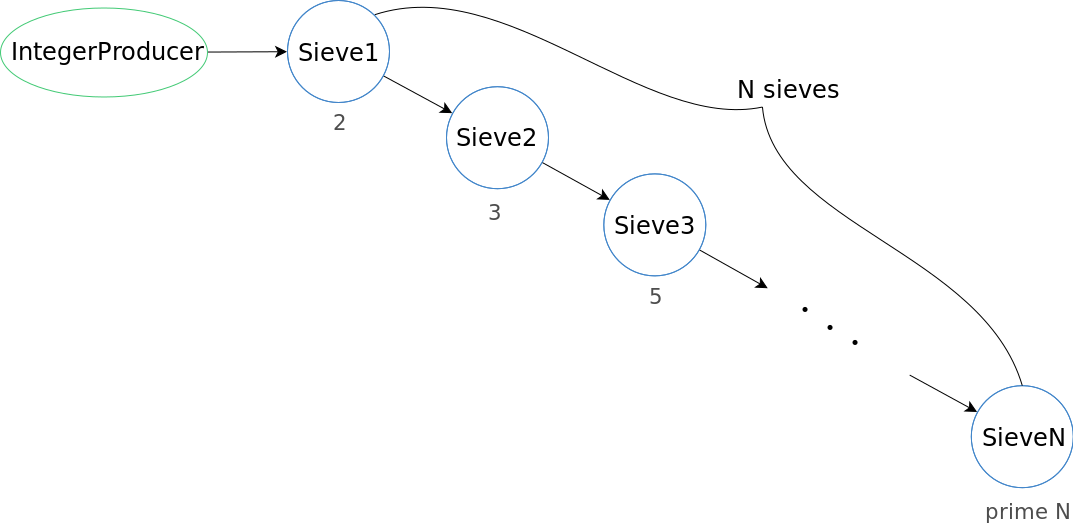
\includegraphics[width=0.8\textwidth]{figures/sieve_static}
	\caption{Workflow for the prime sieve}	\label{fig:sieve_static}
\end{figure}

To define the graph, we need exactly two numbers: one is the range (\ie the maximum number) and the other is the number of primes in this region. Typically, we need to first find out the number of primes in this range by running a prime generator elsewhere, and then use it to construct the workflow. If we set the number smaller, the workflow can execute, but will produce unreliable numbers when the actual number of primes exceeds the number of sieves defined in the workflow graph; if we set the number larger, the correctness of the workflow execution will then depend on how outputs from the sieves are connected to the successor nodes (e.g. if only the final sieve is connected to the successor nodes, then there will be no outputs from the last sieve and, therefore, no inputs to the successor so it will behave erroneously).

Two problems emerge from this construction method:
\begin{enumerate}
	\item The recursive dependency problem previously mentioned;
	\item A different graph is needed when we want to change the maximum number.
\end{enumerate}

Both of them are quite unsatisfying for researchers / developers because they both involve manual inspection apart from the basic workflow (especially task) design. Researchers, \eg us, would prefer a more unified automatic way in which we only need to define once without calculating the number of primes before execution.

This motivates our research and we present the new semantics called \emph{dynamic expansion} (in addition to \emph{incremental deployment}) to support this expectation. In the new semantics, we no longer need to manually assign many sieves. Instead, we only need to define the \cdSieve automatically expandable (by setting the \lstinline|repeatable| property to \lstinline|True|) and describe when to expand it (by connecting \lstinline|circuit|). Moreover, in our new system, another new use case is available: to find certain number of primes -- by making the \cdSieve nodes aware of their status and no longer expand more sieves (it will be more efficient if \emph{backward shut-down propagation} is implemented). Details will be described in the Dynamic Expansion chapter.

\section{Seismic cross-correlation}
Cross-correlation is a method used in seismology to process data from the observers (\eg sensors from stations) by comparing (\ie making calculations of) data of each pair of sensors / sources / stations. Performing cross-correlation is unavoidable for the development of many reliable seismic risk assessment methods \cite{doi:10.1177/1094342016649766}.

\begin{figure}[h]
\centering
    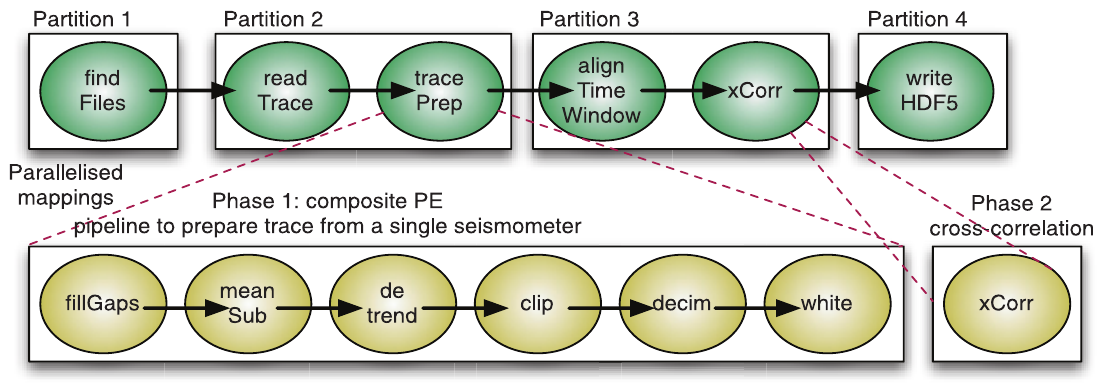
\includegraphics[width=0.8\textwidth]{figures/wf_xcorr}
\caption{Illustration of the cross-correlation workflow by \citeauthor{doi:10.1177/1094342016649766}\cite{doi:10.1177/1094342016649766}}
\label{fig:wf_xcorr}
\end{figure}

\citeauthor{doi:10.1177/1094342016649766}\cite{doi:10.1177/1094342016649766} presented an illustration (see Figure \ref{fig:wf_xcorr}) to the structure of the cross-correlation (xcorr) workflow. Apart from the reading and writing of files, it contains two steps: preprocess and cross-correlation. The preprocess step reads data from stations and performs some preprocess. The raw data is very large but the preprocessed data is smaller than that. Each trace (data from one station) can be preprocessed independently, and the preprocessed data are fed into many cross-correlations PEs.

Because the preprocess step requires online station data, it is better for us to cache the data on local disks when performing evaluation. Because the raw data amount is large and is largely reduced after preprocessing, we cache the preprocessed data on local disks and only performs the cross-correlation step to evaluate the performance. This does not affect the ability to demonstrate because cross-correlation is also highly parallelizable -- it performs actions on each pair of stations so the total number of cross-correlation (independent with each other) is $C^2_n$ for $n$ traces where $C^k_n$ represents the number of $k$ combinations in $n$ elements, and hence $C^2_n=\frac{n(n-1)}{2}$.

The workflow\footnote{Originates from \url{https://github.com/rosafilgueira/dispel4py_workflows}.} we use consists of four \tPETmpl{}s and can be decomposed into two partitions (see Figure \ref{fig:wf_xcorr_us}). The four \tPETmpl{}s are:

\begin{figure}[h]
\centering
    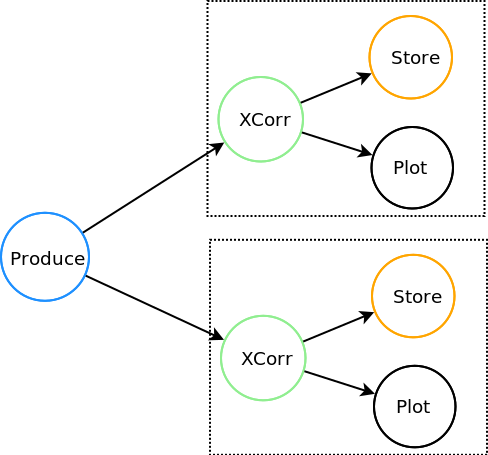
\includegraphics[width=0.8\textwidth]{figures/wf_xcorr_us}
\caption{Illustration of the cross-correlation workflow we use}
\label{fig:wf_xcorr_us}
\end{figure}

\begin{enumerate}
	\item \lstinline|Producer| which reads (pre-processed) data from disk and stream them to \lstinline|XCorr|.
	\item \lstinline|XCorr| reads data and performs cross-correlation until no more data is coming in. It sends the processed data to both \lstinline|Store| and \lstinline|Plot|.
	\item \lstinline|Store| saves data to disk.
	\item \lstinline|Plot| produces a plot (to the disk) of the data.
\end{enumerate}

Each \lstinline|XCorr| is associated with one \lstinline|Store| and one \lstinline|Plot| and they forms a partition. The cross-correlation itself is computation-intensive, but highly parallelizable. Therefore, this partition can be duplicated for many times for better parallelism and would get better performance.

The plot step is not a part of the computation of cross-correlation, but is a step for visualization. It consumes a lot of time especially when the number of cross-correlations is large. We keep it in the workflow for a few traces, but remove it for larger numbers of traces (\eg over 100).
